
\documentclass[sigconf, nonacm]{acmart}
\AtBeginDocument{\providecommand\BibTeX{{Bib\TeX}}}

\usepackage{verbatim}
\usepackage[linesnumbered, boxed, resetcount]{algorithm2e}
\usepackage{subcaption}

\settopmatter{printfolios=true} 

\begin{document}

\title{}
\title[SPHEROID METRICS]{SPHEROID METRICS: Automated Segmentation and Morphological Analysis of Cancer Spheroids in Bright-Field Images}

\author{Tulasi Rajgopal, Richard VanWinkle, Sara Prasla}

\affiliation{
  \institution{University of Applied Sciences Würzburg-Schweinfurt (THWS)}
  \city{Würzburg}
  \country{Germany}
}

\renewcommand{\shortauthors}{Rajgopal, VanWinkle, Prasla}

\begin{abstract}
Pancreatic cancer remains highly lethal and difficult to treat, motivating the use of three-dimensional spheroid models that accurately capture tumor growth and drug response compared to conventional monolayer cultures. Variability in spheroid shape, imaging conditions, and debris further limits the reliability and reproducibility of manual and semi-automated approaches, which are time-consuming and subjective. Despite these challenges, quantitative morphological metrics derived from these spheroids provide critical insight into treatment effects.

This work presents an automated image-analysis pipeline for spheroid segmentation and morphological quantification using bright-field microscopy spheroid images. The approach employs deep learning–based segmentation models, including YOLOv8 segmentation and U-Net, to robustly delineate spheroid boundaries under challenging imaging conditions. Following segmentation, the pipeline extracts key morphological and intensity-based metrics such as relative area, circularity, and gray-level co-occurrence matrix (GLCM) features to enable comparatively fast and scalable assessment of tumor growth and drug efficacy in 3D cancer models.
\textbf{Keywords:} Three-dimensional (3D) spheroids; in vitro models; in vivo relevance; image segmentation; morphological metrics

\end{abstract}

\maketitle
%% Add here the link to your code repository
\vspace{-0.5em}
\textbf{Code:} \url{https://github.com/thws-mai/PM25_Efficacy}

\section{Introduction}\label{introduction}
Pancreatic cancer remains one of the deadliest malignancies, characterized by late diagnosis, rapid progression, and limited therapeutic response \cite{ref12}. Preclinical evaluation of drug efficacy increasingly relies on three-dimensional (3D) tumor spheroid models grown in vitro (outside a living organism under controlled laboratory conditions), which more accurately reflect aspects of the in vivo tumor microenvironment (within a living organism) than traditional two-dimensional cultures \cite{ref1}. Spheroids preserve critical biological characteristics, including cell–cell interactions, nutrient gradients, hypoxia, and drug penetration profiles \cite{ref1}, making them well suited for studying tumor growth dynamics and treatment response.

Quantitative analysis of spheroid morphology from bright-field microscopy images plays a central role in assessing drug-induced effects such as growth inhibition, structural degradation, and changes in cellular viability. Reliable measurement of these effects requires accurate segmentation of spheroid boundaries to separate tumor regions from background and imaging artifacts. However, manual annotation and measurement remain labor-intensive, subjective, and difficult to reproduce, particularly in longitudinal and high-throughput studies. Variability in imaging conditions, irregular spheroid morphologies, debris, and low contrast between spheroids and the background further complicate consistent segmentation and metric extraction, limiting scalability and reproducibility.

Recent advances in deep learning–based image segmentation provide effective tools for automating spheroid boundary detection and enabling systematic morphological analysis. Nevertheless, existing approaches often exhibit important limitations. Many recent pipelines rely on fluorescence imaging to infer viability or cell composition \cite{ref3,ref8}, which increases experimental complexity and requires labeling and staining. Other methods focus primarily on detection or segmentation and leave quantitative analysis to the user \cite{ref4}, while some end-to-end convolutional models learn abstract features that are difficult to interpret biologically \cite{ref9}. These limitations restrict the adoption of automated spheroid analysis in routine bright-field assays.

In this work, we present an end-to-end automated pipeline for spheroid segmentation and quantitative analysis in bright-field microscopy images using YOLOv8 segmentation and U-Net architectures \cite{ref4,ref5}. The pipeline integrates robust data pre-processing and augmentation, enables accurate spheroid boundary delineation under challenging imaging conditions, and supports automated extraction of biologically relevant morphological, intensity, and texture-based metrics to quantify spheroid growth changes and drug-induced effects. The proposed framework serves as a baseline, robust, and interpretable analysis tool for bright-field spheroid assays and functions as a first-line screening approach prior to more complex or modality-specific analyses, supporting scalable and reproducible evaluation in preclinical cancer studies.

\section{Related work}\label{relatedwork}
Early approaches to spheroid image analysis rely on manual annotation or classical image processing techniques \cite{ref1}. Manual measurement provides direct control but remains subjective and impractical for large datasets or longitudinal studies. Classical methods based on thresholding or edge detection offer partial automation but struggle under variable imaging conditions, irregular spheroid morphologies, and low contrast commonly observed in bright-field microscopy images.

Recent advances in deep learning significantly improve spheroid detection and segmentation performance. Convolutional neural networks, particularly U-Net–based architectures, demonstrate strong capability in biomedical image segmentation \cite{ref2} by capturing multiscale spatial features. Object detection and segmentation frameworks such as YOLO further enable efficient localization and boundary delineation of spheroids in complex scenes. These learning-based methods improve robustness compared to traditional approaches and support automated processing across diverse datasets.

However, several recent deep learning–based pipelines address only limited aspects of spheroid analysis. Many approaches operate on fluorescence microscopy images for predicting cell viability or population fractions, which increases experimental complexity and requires labeling \cite{ref8}. Other methods focus primarily on spheroid detection or segmentation and leave quantitative morphological analysis entirely to the user \cite{ref4}. Several end-to-end convolutional models produce global predictions or learned feature representations that are difficult to interpret biologically \cite{ref9}. 

These limitations highlight the need for automated spheroid analysis frameworks that operate directly on bright-field images, integrate robust segmentation with interpretable metric extraction, and support scalable and reproducible analysis. The proposed work builds upon recent deep learning advances while addressing practical gaps in usability, interpretability, and quantitative assessment for preclinical cancer studies.

\section{Dataset and Preprocessing}\label{dataprocessing}

%\subsection{Dataset Description}

We use bright-field microscopy images of PDAC (pancreatic ductal adenocarcinoma) spheroids acquired under controlled and drug-treated conditions \cite{ref10}. The primary dataset consists of 179 fully annotated images with YOLO-format labels, in which spheroid boundaries are encoded as polygon-based regions for object localization and segmentation. This dataset is used for training and validation of the segmentation models, and all annotations are verified to ensure accurate boundary alignment and exclusion of non-spheroid artifacts.

A second dataset includes 60 paired PDAC spheroid samples, each with one untreated control image and one image treated with a drug combination (JQ1 and GANT61). This dataset contains no annotations and is used exclusively for model inference, metric extraction, and comparative analysis between control and treated conditions. It is not used during training or validation.

%\subsection{Annotation Conversion and Organization}
For U-Net training, the polygon-based YOLO annotations are converted into pixel-wise binary segmentation masks, where each pixel is explicitly labeled as spheroid or background, in contrast to the region-based annotation format used by YOLO. We organize images and corresponding masks into structured directories to ensure reproducibility and support collaborative workflows. We match each image–mask pair using consistent filename conventions to prevent misalignment during data loading and training.

%\subsection{Preprocessing Pipeline and Data Augmentation}

The limited availability of annotated training data constrains robust deep learning–based segmentation. To mitigate this limitation and improve model generalization, we apply a controlled data augmentation strategy during training. Specifically, we perform horizontal and vertical flipping, as well as rotations by 90° and 270°. These transformations preserve spheroid morphology while increasing the effective diversity of the training dataset.

The preprocessing pipeline includes the following steps:
 \begin{enumerate}
 \item Matching images from the image directory with corresponding segmentation masks from the label directory.

\item The dataset is partitioned into training, validation, and test sets directories with the ratio of 70/15/15, respectively using filename suffix–based grouping to ensure that augmented versions of the sample remain within the respective subset.

\item Resizing images and masks to fixed spatial dimensions (512 × 512 for U-Net or 768 × 768 for YOLOv8n) using uniform scaling.

\item Pixel intensity normalization using mean and standard deviation calculated from the dataset images with the custom code.

\item Batch loading for efficient model training.
  
 \end{enumerate}

 %\subsection{Preprocessing of Unannotated Experimental Data}

A separate preprocessing pipeline is applied to the unannotated experimental dataset, which includes spheroid images acquired under varying magnification, framing, and illumination conditions. These differences introduce additional challenges for direct inference and metric extraction.

To address these variations, the following steps are applied exclusively to the unannotated dataset:

\begin{enumerate}
    \item Automated spheroid localization using coarse model inference combined with intensity-based heuristics.
    
    \item Centered zoom-cropping around detected spheroid regions to remove excess background and peripheral debris, followed by rescaling to match the spatial resolution used during training.
    
       

\end{enumerate}

These preprocessing operations are strictly isolated from the training and validation pipelines to preserve the integrity of model evaluation.

\section{Methodology}\label{methodology}
%\subsection{Design Objectives and Challenges}\label{challenges}

The objective of this work is to achieve accurate spheroid boundary segmentation that enables reliable extraction and comparison of morphological and intensity-based metrics for assessing spheroid growth changes and drug-induced effects. This task is constrained by a limited amount of annotated training data, the presence of debris and low-contrast backgrounds, irregular and evolving spheroid morphologies, and variability in image acquisition conditions between control and treated samples. These challenges require segmentation models that are robust to noise, preserve boundary fidelity, and generalize well under limited supervision.

To address these constraints, we investigate two complementary deep learning–based segmentation approaches, namely YOLOv8 segmentation and a U-Net architecture, and evaluate their suitability for downstream biological analysis. We perform model selection based on segmentation quality, as discussed in Section~\ref{eval_results}.


%\subsection{YOLOv8-Based Instance Segmentation}

We train a YOLOv8n-seg model to perform automated spheroid detection and instance-level segmentation on bright-field microscopy images. YOLOv8 is selected for its unified detection--segmentation formulation, high inference efficiency, and robustness in cluttered scenes under limited annotated data. These properties are particularly important for spheroid images containing debris, merged objects, and heterogeneous backgrounds.

The model is trained for 1000 epochs using the Ultralytics YOLOv8 training pipeline with an input resolution of $768 \times 768$. Batch size is selected based on available hardware resources. Conservative, boundary-preserving augmentations are applied during training, including mild Gaussian blur ($p = 0.20$), while aggressive intensity normalization and brightness or contrast jitter are avoided to preserve boundary consistency in low-contrast regions.
YOLOv8 optimizes a composite objective $L = L_{\text{box}} + L_{\text{cls}} + L_{\text{mask}} + L_{\text{dfl}}$, where the classification and mask terms minimize binary cross-entropy (negative log-likelihood), i.e., $L_{\text{cls}} = -\sum_i \left[y_i \log(p_i) + (1-y_i)\log(1-p_i)\right]$ and $L_{\text{mask}} = -\sum_{x,y} \left[m_{xy}\log(\hat{m}_{xy}) + (1-m_{xy})\log(1-\hat{m}_{xy})\right]$. The bounding-box component $L_{\text{box}}$ minimizes an IoU-based regression loss, and $L_{\text{dfl}}$ refines box coordinates via Distribution Focal Loss. This formulation enforces accurate localization and stable instance masks, which directly support reliable downstream morphological measurements such as area and perimeter under heterogeneous imaging conditions.


%\subsection{U-Net--Based Pixel-Wise Segmentation}

To achieve higher boundary precision and shape preservation, we employ a U-Net--based fully convolutional network \cite{ref2} for pixel-wise spheroid segmentation. The architecture follows a standard encoder--decoder design with symmetric skip connections, enabling accurate spatial localization while retaining contextual information. This design is critical for spheroid segmentation, where small boundary errors directly affect downstream metrics such as perimeter, circularity, and area.

Given the limited availability of annotated training data, a ResNet34 encoder with pretrained weights is employed to improve feature generalization and mitigate overfitting. The U-Net model is trained for 30 epochs using images resized to \(512 \times 512\) pixels, a resolution that balances boundary detail preservation with computational efficiency. We perform optimization using the Adam optimizer with a learning rate of \(1 \times 10^{-4}\), providing stable convergence during training.

Accurate segmentation of bright-field spheroid images requires not only pixel-wise classification accuracy but also precise boundary alignment and size preservation to enable reliable morphological and intensity-based metric measurement. Although region-based losses such as Dice are widely used for binary cell segmentation, prior work reports that Dice loss provides limited gradient feedback and does not consistently outperform distribution-based losses such as cross-entropy, particularly when boundary precision is critical \cite{ref7}. Motivated by these findings and the presence of boundary ambiguity, debris, and irregular spheroid morphology, we employ a multi-term loss function defined in Eq.~\ref{unet_loss}. The Binary Cross-Entropy term
$L_{\mathrm{BCE}} = -\frac{1}{N}\sum_{i}\left[y_i \log(p_i) + (1 - y_i)\log(1 - p_i)\right]$
provides stable pixel-wise supervision and detailed gradient signals. The IoU-based overlap loss
$L_{\mathrm{IoU}} = 1 - \mathrm{IoU}$
promotes global region consistency under class imbalance. To explicitly penalize edge misalignment, a boundary IoU loss
$L_{\mathrm{Boundary}} = 1 - \mathrm{BIoU}$
is incorporated and assigned a higher weight, as small boundary errors disproportionately affect perimeter- and circularity-based metrics. Finally, an area-matching loss
$L_{\mathrm{Area}} = \frac{\left|A_{\mathrm{pred}} - A_{\mathrm{gt}}\right|}{A_{\mathrm{gt}} + \epsilon}$
constrains relative size deviations, discouraging over- and under-segmentation and preserving biologically meaningful spheroid size. This composite formulation avoids reliance on a single region-based objective and directly enforces the segmentation properties required for robust downstream morphological and intensity-based analysis.
\begin{equation}
\label{unet_loss}
L = \alpha_{\mathrm{BCE}} L_{\mathrm{BCE}} + \alpha_{\mathrm{IoU}} L_{\mathrm{IoU}} + \alpha_{\mathrm{Boundary}} L_{\mathrm{Boundary}} + \alpha_{\mathrm{Area}} L_{\mathrm{Area}}
\end{equation}

\begin{figure}[htbp]
    \centering
    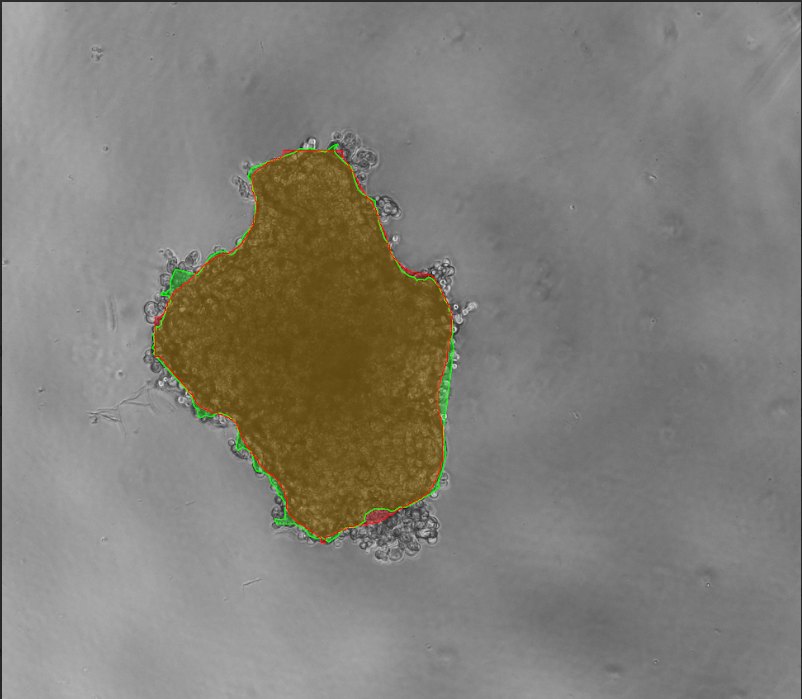
\includegraphics[width=0.46\linewidth]{yoloresult.png}
    \hfill
    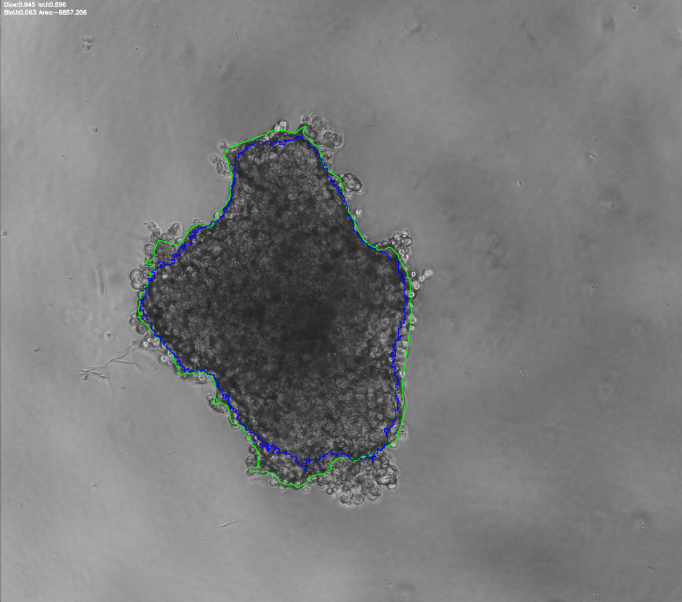
\includegraphics[width=0.46\linewidth]{unet result.png}
    {\footnotesize
    \caption{Qualitative comparison of spheroid segmentation using YOLOv8 (left) and U-Net (right). Ground-truth boundaries are shown in green, YOLOv8 predictions in red, and U-Net predictions in blue. The figure highlights differences in boundary adherence and instance coherence under heterogeneous imaging conditions, illustrating YOLOv8’s robustness to debris and low-contrast regions, which directly impacts the stability of downstream morphological measurements.}
    }
    \label{fig:comparison}
\end{figure}

YOLOv8 provides robust instance-level segmentation under cluttered and heterogeneous imaging conditions, while U-Net emphasizes fine-grained boundary accuracy and shape preservation. Both models generate segmentation masks used for automated extraction of morphological and intensity-based metrics. Model selection is based on comparative segmentation quality and the stability of downstream metric measurements.

 %\subsection{Postprocessing}
To improve the reliability of downstream metric extraction, predicted segmentation masks are post-processed to suppress isolated regions and enforce structural consistency. In a small subset of treated samples, low contrast and dark background regions occasionally produce fragmented or weakly connected predictions, particularly near indistinct spheroid boundaries. Morphological opening and closing operations reduce such artifacts, while connected-component filtering removes small, non-spheroid regions, ensuring that retained masks correspond to contiguous and biologically plausible spheroid structures.


%\subsection{Automated Analysis Pipeline}

The automated analysis pipeline integrates segmentation and quantitative analysis and proceeds through data ingestion and preprocessing, model inference for spheroid mask generation, post-processing to remove artifacts and isolate valid regions, feature extraction from segmented spheroids, and statistical comparison between control and treated samples. Steps related to data preparation, inference, and mask refinement are described in Sections~\ref{dataprocessing} and~\ref{methodology}, while feature extraction and comparative analysis are detailed in Section~\ref{metrics}.


\section{Feature Extraction and Metrics}\label{metrics}
Quantitative assessment of spheroid growth and drug response requires features that are both biologically interpretable and robust to imaging variability. We extract complementary sets of morphological and texture-based metrics from the segmented spheroid regions. %Morphological metrics capture global changes in size and shape that directly reflect growth inhibition and structural degradation, while texture metrics characterize internal intensity patterns associated with heterogeneity and treatment-induced disruption.%

%\subsection{Morphological Metrics}

Morphological metrics are extracted from the segmented spheroid masks to quantify changes in spheroid size, shape, and structural integrity following drug treatment. These features provide direct and interpretable indicators of growth suppression and cytotoxic effects and are widely used in spheroid-based assays \cite{ref10,ref11}.

Area quantifies spheroid size as the total number of pixels within the segmented region and is computed as $A = \sum_{x,y} M(x,y)$, where $M(x,y) \in \{0,1\}$ denotes the binary mask. Differences in area between control and treated samples reflect growth inhibition or structural disintegration. Perimeter measures boundary length and captures edge irregularity, where disproportionate increases relative to area indicate reduced compactness. Circularity, defined as $\text{Circularity} = \frac{4\pi \cdot \mathrm{Area}}{\mathrm{Perimeter}^2}$, quantifies deviation from an ideal circular shape, with lower values indicating morphological instability. Together, these metrics characterize size, boundary complexity, and structural integrity for objective comparison between conditions.


%\subsection{Texture Metrics Using Gray-Level Co-occurrence Matrix (GLCM)}

While morphological metrics describe global shape changes, they do not capture internal intensity variations that reflect spheroid heterogeneity and treatment-induced disruption. To address this, we extract texture features using the Gray-Level Co-occurrence Matrix (GLCM) \cite{ref6}, which characterizes spatial intensity relationships within the spheroid region and is robust to global brightness variations.

Given a quantized grayscale image with $N_g$ gray levels, the GLCM $P(i,j \mid d,\theta)$ represents the normalized co-occurrence frequency of intensity levels $i$ and $j$ at pixel distance $d$ and orientation $\theta$. Each image is converted to grayscale, quantized to $N_g = 32$ levels, and analyzed only within the predicted spheroid region. To reduce boundary-related artifacts, the spheroid mask is eroded by three pixels, and masked-out pixels are excluded from computation.

Symmetric, normalized GLCMs are computed for distances $d \in \{1,2,4\}$ and orientations $\theta \in \{0^\circ, 45^\circ, 90^\circ, 135^\circ\}$. Texture metrics are reported as the mean across all $(d,\theta)$ combinations. We extract Energy ($\sum_{i,j} P(i,j)^2$), Entropy ($-\sum_{i,j} P(i,j)\log_2(P(i,j)+\epsilon)$), and Contrast ($\sum_{i,j}(i-j)^2P(i,j)$), which collectively capture uniformity, randomness, and local intensity variation within the spheroid.

Because GLCM-based features depend on relative intensity co-occurrence patterns rather than absolute brightness values, they enable consistent comparison between control and treated spheroids under varying illumination and acquisition conditions.

\begin{figure}[htbp]
    \centering
    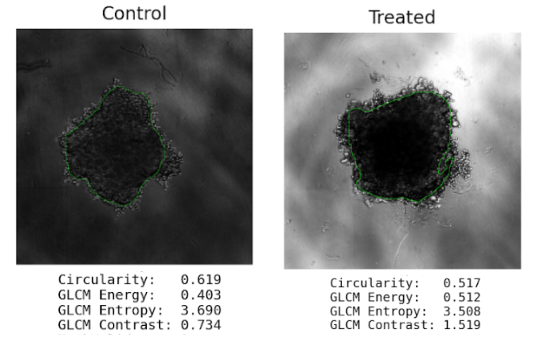
\includegraphics[width=0.93\linewidth]{figure2.png}
    {\footnotesize
    \caption{Comparison of circularity and GLCM-derived texture metrics between control and drug-treated spheroids obtained using YOLOv8 segmentation. Treated samples exhibit reduced structural regularity and altered texture characteristics, indicating drug-induced morphological disruption captured by the proposed segmentation and analysis pipeline.}
    }
\end{figure}
\section{Experimental Results and Evaluation}\label{eval_results}
Segmentation performance is evaluated to determine suitability for stable and interpretable metric extraction rather than to maximize segmentation accuracy alone. Evaluation focuses on region overlap, i.e., $\mathrm{IoU}=\frac{|P \cap G|}{|P \cup G|}$ (where $P$ is the predicted mask and $G$ is the ground-truth mask), as well as boundary fidelity and area preservation, which directly affect morphological and intensity-based measurements.

YOLOv8 achieves a mean IoU of 92\% and an average ground truth–to–prediction area ratio of 99\%, indicating accurate spheroid localization and strong size preservation across control and treated samples, while remaining robust in cluttered and low-contrast conditions. The U-Net model attains a mean IoU of 0.90, demonstrating strong region overlap and smoother boundaries in high-contrast cases; however, boundary ambiguity under low contrast and occasional misalignment affect perimeter-sensitive measurements, reflected in reduced Boundary IoU and increased variability in area agreement. Given the emphasis on reliable region isolation and metric stability, YOLOv8 is selected for subsequent analysis, prioritizing robustness and consistency over marginal boundary smoothness improvements.

For comparative analysis between control and treated spheroids, only circularity is considered from the morphological category \cite{ref11}, and texture-based metrics derived from the Gray-Level Co-occurrence Matrix as these metrics are unitless and normalized, which mitigates variability introduced by time-dependent and environmental factors, such as changes in illumination during image acquisition.

Overall, the evaluation confirms that reliable segmentation directly supports stable extraction of interpretable, unitless features, enabling consistent assessment of spheroid growth changes and drug-induced effects in bright-field assays.
\section{Conclusion and Future Work}\label{conclusion}

This work presents a reliable and automated framework for analyzing pancreatic cancer spheroids from bright-field microscopy images, with the goal of supporting quantitative assessment of spheroid growth and drug-induced changes under limited annotated data and variable imaging conditions. As accurate segmentation is a prerequisite for downstream analysis, we evaluate two deep learning–based segmentation approaches, U-Net and YOLOv8n, for robust spheroid boundary detection. While both models demonstrate comparable performance, YOLOv8n achieves slightly higher mean IoU and exhibits greater robustness to background clutter and imaging variability. Based on these observations, YOLOv8n is selected as the final segmentation model.

Building on the selected segmentation output, we extract morphological and intensity-based features to quantify treatment-induced changes in spheroid structure. To enable reliable comparison between control and treated samples acquired at different time points and under varying environmental conditions, we focus on unitless and relative metrics. In particular, circularity and texture features derived from the Gray-Level Co-occurrence Matrix are selected, as they directly reflect structural degradation and internal heterogeneity while remaining biologically interpretable. Together, these steps form a simple, robust, and reproducible pipeline for spheroid-based drug efficacy analysis.

While the selected metrics capture meaningful morphology-driven changes, they do not describe complex biological mechanisms such as invasive behavior or multilayer organization. Accordingly, the proposed framework is intended as a baseline and interpretable first-line screening tool for bright-field spheroid assays rather than a comprehensive mechanistic analysis platform.

The current implementation targets technically proficient users who can operate the analysis pipeline directly. Future work will focus on developing a user-friendly interface to enable broader adoption in preclinical drug evaluation studies and on extending the framework to support longitudinal spheroid analysis across multiple time points.


\begin{thebibliography}{00}

\bibitem{ref1}
A. Friedrich et al., ``Spheroid-based tumor models for drug testing,'' \emph{Nature Protocols}, 2009.

\bibitem{ref2}
O. Ronneberger, P. Fischer, and T. Brox,
``U-Net: Convolutional Networks for Biomedical Image Segmentation,''
\emph{MICCAI}, 2015.

\bibitem{ref3}
F. Bresciani et al., ``A brightfield cell viability model using deep learning,'' \emph{Cells}, 2019.


\bibitem{ref4}
A. Akshay et al., ``SpheroScan: a user-friendly deep learning tool for spheroid image analysis,'' \emph{GigaScience}, 2023.


\bibitem{ref5}
M. Streller et al., ``Image segmentation of treated and untreated tumor spheroids by fully convolutional networks,'' \emph{arXiv preprint}, 2024.


\bibitem{ref6}
R. M. Haralick, K. Shanmugam, and I. Dinstein, ``Textural Features for Image Classification,''
\emph{IEEE Transactions on Systems, Man, and Cybernetics}, 1973.

\bibitem{ref7}
C. H. Sudre, W. Li, T. Vercauteren, S. Ourselin, and M. J. Cardoso,
``Generalised Dice overlap as a deep learning loss function for highly unbalanced segmentations,''
\emph{Deep Learning in Medical Image Analysis (DLMIA)}, 2017.

\bibitem{ref8}
A. K. Mali et al., ``A deep learning pipeline for morphological and viability assessment of 3D cancer cell spheroids,'' \emph{Biology Methods and Protocols}, 2025.

\bibitem{ref9}
Z. A. Sheikh et al., ``Deep learning for predicting spheroid viability: Novel convolutional neural network model for automating quality control for three-dimensional bioprinting,'' \emph{Bioengineering}, 2021.

\bibitem{ref10}
Z. Wen et al., ``A spheroid-based 3-D culture model for pancreatic cancer drug testing, using the acid phosphatase assay,'' \emph{Brazilian Journal of Medical and Biological Research}, vol.~46, no.~7, pp.~634--642, 2013.

\bibitem{ref11}
K. Zeeberg et al., ``Assessment of different 3D culture systems to study tumor phenotype and chemosensitivity in pancreatic ductal adenocarcinoma,'' \emph{International Journal of Oncology}, vol.~49, no.~1, pp.~243--252, 2016.

\bibitem{ref12}
M. Hidalgo et al., ``Pancreatic cancer,'' \emph{New England Journal of Medicine}, vol. 362, no. 17, pp. 1605--1617, 2010.

\end{thebibliography}
\end{document}